\documentclass[12pt]{article}
\usepackage{authblk}
\usepackage{upgreek}
\usepackage{multirow}
\usepackage{indentfirst}
\usepackage{setspace}
\usepackage{geometry}
\usepackage{graphicx}
\usepackage{newtxtext, newtxmath}
\geometry{a4paper,left=2.45cm,right=2.45cm,top=2.45cm,bottom=2.45cm}
\title{\huge Design and Analysis of a Laminated Composite Tube}
\author{Jiatai Deng, Jiawei Shuang, Xuanye Hu}
\affil{Department of Mechanical, Aerospace and Civil Engineering}
\date{\today}
\newpage
\begin{document}
\newpage
\maketitle
\thispagestyle{empty}
\newpage
\tableofcontents
\thispagestyle{empty} 
\newpage

\section{General description and requirement}
\setcounter{page}{1}
\pagenumbering{arabic}
\onehalfspacing
\noindent A cylindrical tube of 4 layers of composite with a layup of 
$\left[\alpha\  \beta\  \alpha\  \beta\right]$is to be designed and by winding tapes cut from a UD carbon-epoxy prepreg sheet on to a cylindrical mandrel of a 25mm radius. For the consideration of practicality, the range of these two winding angles will have to fall in [-75°, -30°] or [+30°, +75°] to the axis of the tube. The thickness of the prepreg is 0.25mm. The tube should be made to a length of 300mm.  \newline
\noindent \textbf{Material properties:}\newline
Internal pressure: $q = 3\times10^{6}$ \qquad Axial force: $P = 25 kN$ \newline
Tube radius: $R = 25\times10^{-3}$ \qquad  Tube length $L = 0.3$ \newline
Elastic constant: $E1 = 236 GPa$ \qquad $E2 = 5 GPa$ \qquad $G = 2.6 GPa$ \qquad $\upsilon_{12} = 0.25 GPa$ \newline
Strengths: $\sigma_{1t}^{*} = 3800 MPa$ \qquad $\sigma_{2t}^{*} = 41 MPa$ \qquad $\sigma_{1c}^{*} = 689 MPa$ \qquad $\sigma_{2c}^{*} = 107 MPa$\qquad\qquad\qquad $\tau _{12}^{*} = 69 MPa$ 
\section{Design approach and theory}
\noindent The thickness of each layers is 0.25mm, thickness in the range is between 0.1~1.0 mm can be seen as lamina. So the developed tube is a laminate with layup: $[\alpha /\beta /\alpha /\beta ]$ and the laminate theory can be used for stress analysis.\newline\newline
\noindent \textbf{STEP I: Define the two winding angles:}\newline
\noindent According to the requirement, the winding angle of 4 layers can be defined:\newline
\begin{center}
$-75^{\circ} \leq \alpha \leq -30^{\circ}$ or $75^{\circ} \leq \alpha \leq 30^{\circ}$\end{center}
\begin{center}
$-75^{\circ} \leq \beta \leq -30^{\circ}$ or $75^{\circ} \leq \beta \leq 30^{\circ}$
\end{center}
\noindent \textbf{STEP II: Define the Stress-Strain Relationship $\left[ Q \right]$ :}\newline
According to the Laminar Stress-Strain Relationship in Material coordinate system: \newline$$\left\{ \sigma \right\} = \left[Q \right] \left\{ \epsilon \right\}$$
$$\left\{ \begin{matrix}
    \sigma_1  \\
    \sigma_2  \\
    \tau_{12}  \\
    \end{matrix} \right\} = \left[\begin{matrix}
		Q_{11} & Q_{12} & 0 \\
		Q_{12} & Q_{22} & 0 \\
		0 & 0 & Q_{66} \\
		\end{matrix} \right] \left\{ \begin{matrix}
			\epsilon_1  \\
			\epsilon_2  \\
			\gamma_{12}  \\
			\end{matrix} \right\} = \left[\begin{matrix}
				\frac{E1}{1-\upsilon^2\frac{E2}{E1}} & \frac{\Upsilon E2}{1-\upsilon^2\frac{E2}{E1}} & 0 \\
				\frac{\Upsilon E2}{1-\upsilon^2\frac{E2}{E1}} & \frac{E2}{1-\upsilon^2\frac{E2}{E1}} & 0 \\
				0 & 0 & G \\
				\end{matrix} \right] \left\{ \begin{matrix}
					\epsilon_1  \\
					\epsilon_2  \\
					\gamma_{12}  \\
					\end{matrix} \right\}$$
\noindent \textbf{STEP III: Define the Coordinate transformation $\left[ T \right]$}\newline
\noindent The winding angle of 4 layers of composite: $ \theta = \left( \begin{matrix}
	\alpha  \\
	\beta  \\
	\alpha  \\
	\beta	\\
	\end{matrix} \right)$, the coordinate transformation between (x-y) and (1-2) matrix:$$ \left\{ T \right\} = \left[\begin{matrix}
			\cos^2{\theta} & \sin^2{\theta} & -2\cos{\theta}\sin{\theta} \\
			\sin^2{\theta} & \cos^2{\theta} & 2\cos{\theta}\sin{\theta} \\
			\cos{\theta}\sin{\theta} & -\cos{\theta}\sin{\theta} & cos^2{\theta}-sin^2{\theta} \\
			\end{matrix} \right]$$\newline
\noindent \textbf{STEP IV: Define maximum stress failare criterion}\newline
\noindent According to the maximum stress failure criterion, material will fail when any of the following conditions is violated:
$$\frac{\sigma_1}{\sigma^*_{1t}} \leq 1 \quad if \quad \sigma_1 > 0 \qquad\qquad\qquad \frac{\left| \sigma_1 \right|}{\sigma^*_{1c}} \leq 1 \quad if \quad  \sigma_1 < 0$$
$$\frac{\sigma_2}{\sigma^*_{2t}} \leq 1 \quad if \quad \sigma_2 > 0 \qquad\qquad\qquad \frac{\left| \sigma_2 \right|}{\sigma^*_{2c}} \leq 1 \quad if \quad  \sigma_2 < 0$$
$$\frac{\left| \tau_{12} \right|}{\tau^*_{12}} \leq 1$$\hfill\newline
\noindent \textbf{STEP V: Define Twist angle}\newline
\noindent Tube is fixed at the bottom end and axially compressed at the top. Generator on the tube deforms by an angle $\gamma_{xy}$.
Point $A$ at the top end moves to $A'$ by a distance $\gamma_{xy}L$.
We can get the twist angle of the tube formula:\newline
\begin{minipage}[b]{0.7\linewidth}
	$$\theta = \frac{\gamma_{xy}L}{R}$$\newline\newline
	\end{minipage}
	\hfill
	\begin{minipage}[b]{0.3\linewidth}
		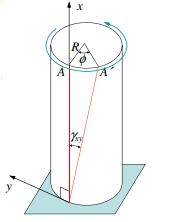
\includegraphics{twist.png}
\end{minipage}
\noindent\textbf{There are two loading conditions, separately analysis:}\newline
\subsection{Case 1: Internal pressure of 3 MPa (ends closed)}
\begin{minipage}[c]{0.5\linewidth}
	\noindent The generalised stresses:
	$ N = \left\{ \begin{matrix}
		N_x=\frac{1}{2}qR \\
		N_y=qR\newline  \\
		N_{xy}=0 
		\right\ }  \\
		\end{matrix} \right\}$\\
\end{minipage}\hfill
\begin{minipage}[c]{0.5\linewidth}
    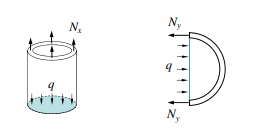
\includegraphics[scale=0.8]{case1.png}
\end{minipage}\hfill\newline
\noindent Generalised stress-strain Relationship:
$ \left\{\begin{matrix}
    N \\
    M \\
    \end{matrix}\right\}=\left[\begin{matrix}
        A\ B\\
        B\ D\\\end{matrix}\right]\left\{\begin{matrix}
        \epsilon^0 \\
        \kappa \\
        \end{matrix}\right\}$,
$\left[A\right]=t\left[T\right]\left[Q\right]\left[T\right]^T$\newline
Strain in x-direction: $\epsilon_x = \left[A\right]^{-1}N$\newline\newline
\noindent Lamina 1: The winding angle is \alpha.\newline
$\epsilon = \left[T_\alpha\right]\left[A\right]^{-1}^T\epsilon_x$\newline
$\sigma = \left[Q\right]\epsilon$\newline
\noindent Lamina 2: The winding angle is \beta.\newline
$\epsilon = \left[T_\beta\right]\left[A\right]^{-1}^T\epsilon_x$\newline
$\sigma = \left[Q\right]\epsilon$\newline
\subsection{Case 2:Axial compression of $P =25 kN$}
\begin{minipage}[c]{0.5\linewidth}
	The generalised stresses:
	$ \left\{ \begin{matrix}
		N_x=\frac{P}{2\pi R}\\
		N_y=0\newline  \\
		N_{xy}=0 
		\right\ }  \\
		\end{matrix} \right\}$
\end{minipage}\hfill
\begin{minipage}[c]{0.5\linewidth}
    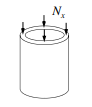
\includegraphics[scale=0.8]{case 2.png}
\end{minipage}\hfill\newline

\section{ Results and analysis to prove the success of the design }

\appendix
\include{appendixA}
\end{document}